\documentclass{article}
\usepackage{tikz}
\usetikzlibrary{automata,positioning}

\begin{document}

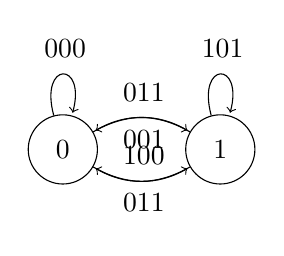
\begin{tikzpicture}[shorten >=1pt,node distance=2cm,on grid,auto]
    \node[state] (q_0) {$0$};
    \node[state] (q_1) [right=of q_0] {$1$};

    \path[->]
        (q_0) edge [loop above] node {$\begin{matrix} 0 \\ 0 \\ 0 \end{matrix}$} ()
              edge [bend left] node {$\begin{matrix} 0 \\ 1 \\ 1 \end{matrix}$} (q_1)
              edge [bend right] node {$\begin{matrix} 1 \\ 0 \\ 0 \end{matrix}$} (q_1)
        (q_1) edge [loop above] node {$\begin{matrix} 1 \\ 0 \\ 1 \end{matrix}$} ()
              edge [bend left] node {$\begin{matrix} 0 \\ 1 \\ 1 \end{matrix}$} (q_0)
              edge [bend right] node {$\begin{matrix} 0 \\ 0 \\ 1 \end{matrix}$} (q_0);
\end{tikzpicture}

\end{document}